%% 公共信息
%%%%%%%%%%%%%%%%%%%%%%%%%%%%%%%%%%%%%%%%%%%%%%%%%%%%%%%%%%%%%%%%%%%%%
\jxdy{%教学单元
  1}
\jxzc{%教学周次
  1}

\dymc{%本次主题
  课程简介 }

\xqfx{%学情分析,每行前面要加 \item
  \item 大一新生;
  \item 多无编程基础和概念;
  \item 无高等数学、大学物理等基础;
  \item 高中学习状态;}

\jxmb{%教学目标,每行前面要加 \item
  \item 什么是C语言;
  \item 为什么学习C语言;
  \item 怎么学C语言;}

\jxzd{%教学重点,每行前面要加 \item
  \item 什么是C语言;
  \item 怎么学C语言;
  \item XXXXX;}

\jxnd{%教学难点,每行前面要加 \item
  \item 怎么学C语言;
  \item C语言概念的泛化;
  \item XXXX;}

\jxff{%教学方法,每行前面要加 \item
  \item 讲述
  \item 举例
  \item 演示}

\jcks{%教材开始页
  123}

\jcjs{%教材结束页
  456}  

\ckks{%参考书开始页
  23}

\ckjs{%cksjshy
  56}
  
\jxhj{%教学后记
     应该加强C语言应用场景的介绍。}

\skrq{%授课日期
  2017年XX月XX日 4-5节}

\makeshouye %授课计划页
%%%%%%%%%%%%%%%%%%%%%%%%%%%%%%%%%%%%%%%%%%%%%%%%%%%%%%%%%%%%%%%%%%%%%

%%%% 教学内容
\subsection{组织教学}%教学内容1级标题
\begin{enumerate}[\hspace{2em}1、]%教学内容列表
  \setlength{\itemsep}{0pt}
  \item 集中学生注意力;
  \item 清查学生人数;\goodmark
  \item 维持课堂纪律;\badmark
\end{enumerate}
  
\subsection{导入及主要内容}
\begin{enumerate}[\hspace{2em}1、]
  \item XXXX;
  \item XXXX;
\end{enumerate}
C语言教学内容的思维导图如 \ref{fig-cmindmap}所示
\begin{figure}[!hbtp]   
        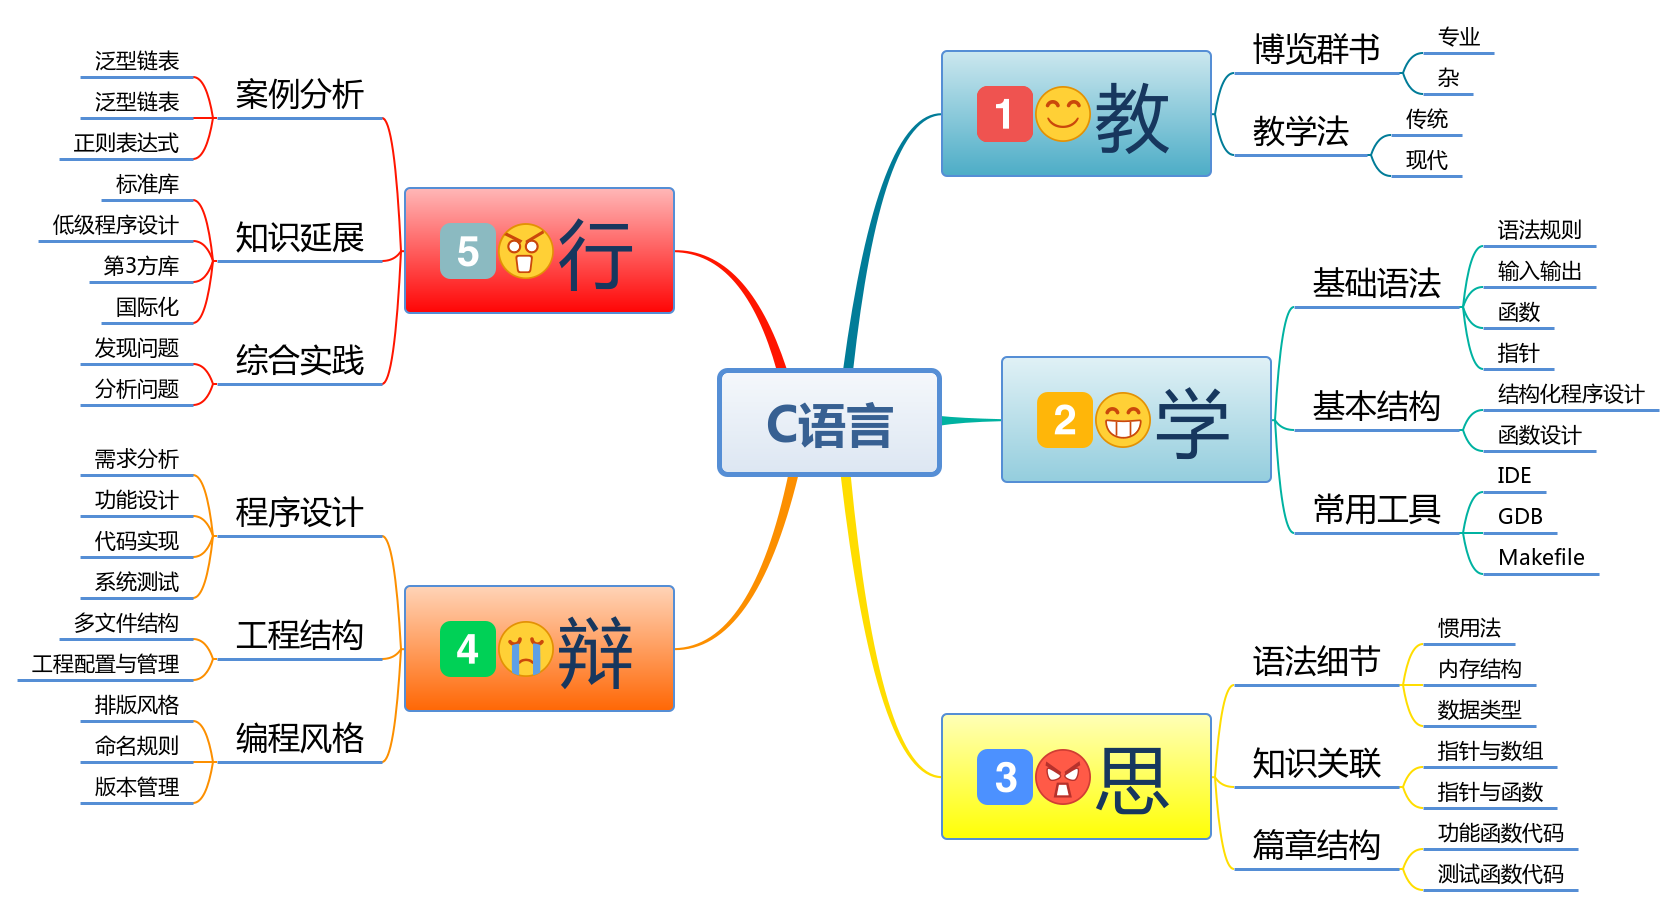
\includegraphics[width=0.6\textwidth]{cprogmindmap} 
        \caption{C语言内容思维导图}\label{fig-cmindmap}
\end{figure}

\subsection{教学内容及过程}
  \subsubsection{本学期期教学安排} \marginpar{说明介绍}%教学内容二级标题,
                                                   % \marginpar用于填写左边框
    \paragraph{理论教学计划:}%教学内容二级标题
    \begin{itemize}
      \item XXXX
      \item XXXX
    \end{itemize}
    \paragraph{实习教学计划}
    \begin{itemize}
      \item XXXX
      \item XXXX
    \end{itemize}
  \subsubsection{教学活动} \marginpar{互动提问}
  \begin{itemize}
    \item XXXX
    \item XXXX
  \end{itemize}

\subsection{课堂小结}
主要介绍了C语言的学习内容和学习方法。\vfill

\subsection{布置作业}
\begin{enumerate}[1、]
  \item XXXX;
  \item XXXX;
\end{enumerate}

\vfill

%%% Local Variables: 
%%% mode: latex
%%% TeX-master: "../main.tex"
%%% End: 
